\begin{frame}{music ai}{opportunities \& threats}
    \vspace{-3mm}
    \begin{columns}
    \column{.5\linewidth}{\textbf{opportunities}}
    
        \begin{itemize}
            \item content creation:
                \begin{itemize}
                    \item speed-up, increased efficiency
                    \item creative possibilities (morphing, etc.)
                    \item co-creative idea givers
                    \item democratization
                \end{itemize}
            \smallskip
            \item consumption:
                \begin{itemize}
                    \item personalization
                    \item effective discovery and accessibility
                \end{itemize}
        \end{itemize}
    \column{.5\linewidth}{\textbf{threats}}
    
        \begin{itemize}
            \item both:
                \begin{itemize}
                    \item 'mainstreamification'
                    \item bias through for-profit system control
                    \item sustainability and energy 
                \end{itemize}
            \item content creation:
                \begin{itemize}
                    \item ethical use of data
                    \item plagiarism growth
                    \item liability for harmful content
                \end{itemize}
            \smallskip
            \item consumption:
                \begin{itemize}
                    \item user distrust through 
                        \begin{itemize}
                            \item inflationary ai-generated content
                            \item inexplainable block-box systems
                        \end{itemize}
                \end{itemize}
        \end{itemize}
        %\vspace{20mm}
        %\begin{figure}%
            %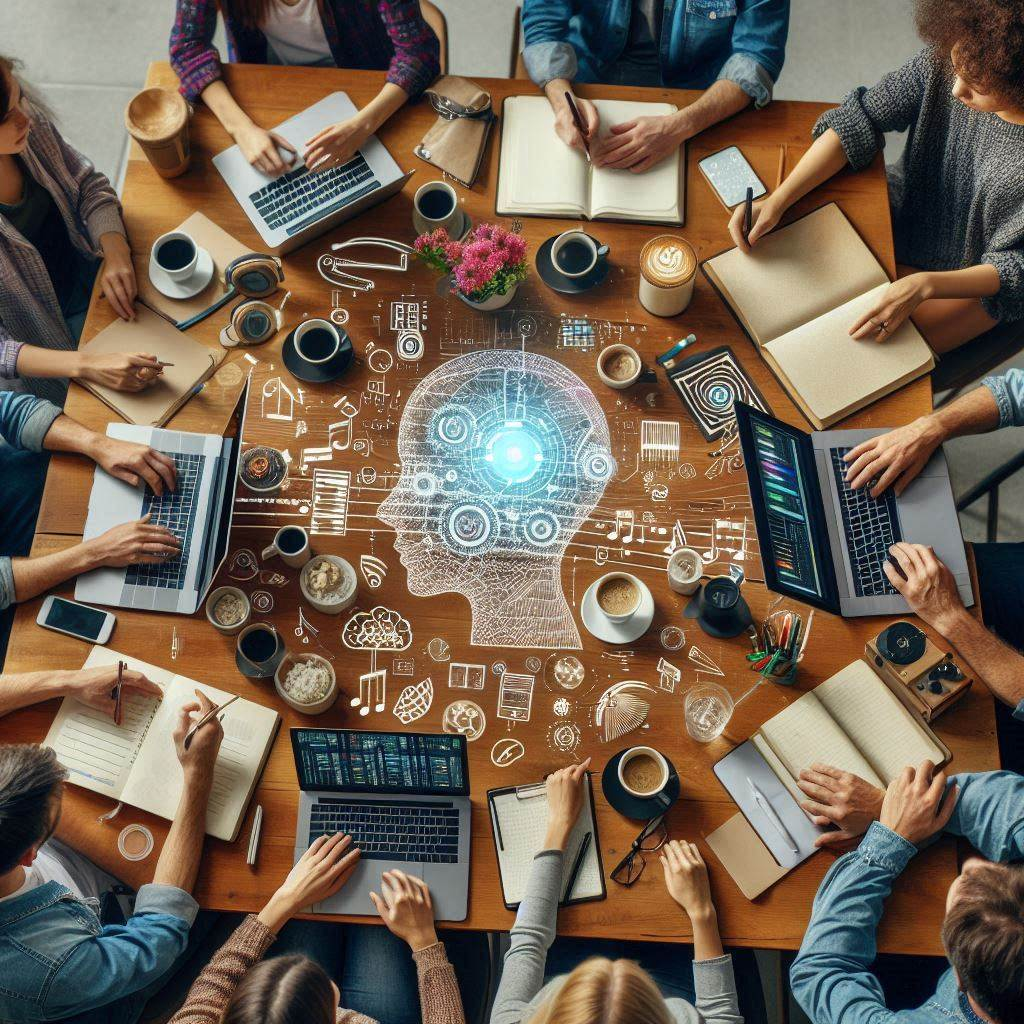
\includegraphics[width=.8\columnwidth]{responsible-ai}%
        %\end{figure}
    \end{columns}
\end{frame}




%\begin{frame}{music ai}{opportunities \& threats 1/2}
    %\vspace{-5mm}
    %\begin{columns}
    %\column{.65\linewidth}
        %\begin{itemize}
            %\item \textbf{ethical considerations}
                %\begin{itemize}
                    %\item training data (copyright, privacy)
                    %\item responsible system usage
                    %\item addressing bias
                %\end{itemize}
            %\smallskip
            %\item \textbf{economic impact}
                %\begin{itemize}
                    %\item understanding the implications for music professionals
                    %\item adapting to new business models and revenue streams
                %\end{itemize}
            %\smallskip
            %\item   \textbf{quality and authenticity}
                %\begin{itemize}
                    %\item plagiarism
                    %\item balancing novelty and predictability/homogeneity
                    %\item hallucination
                %\end{itemize}
            %\smallskip
        %\end{itemize}
    %\column{.35\linewidth}
        %\vspace{20mm}
        %\begin{figure}%
            %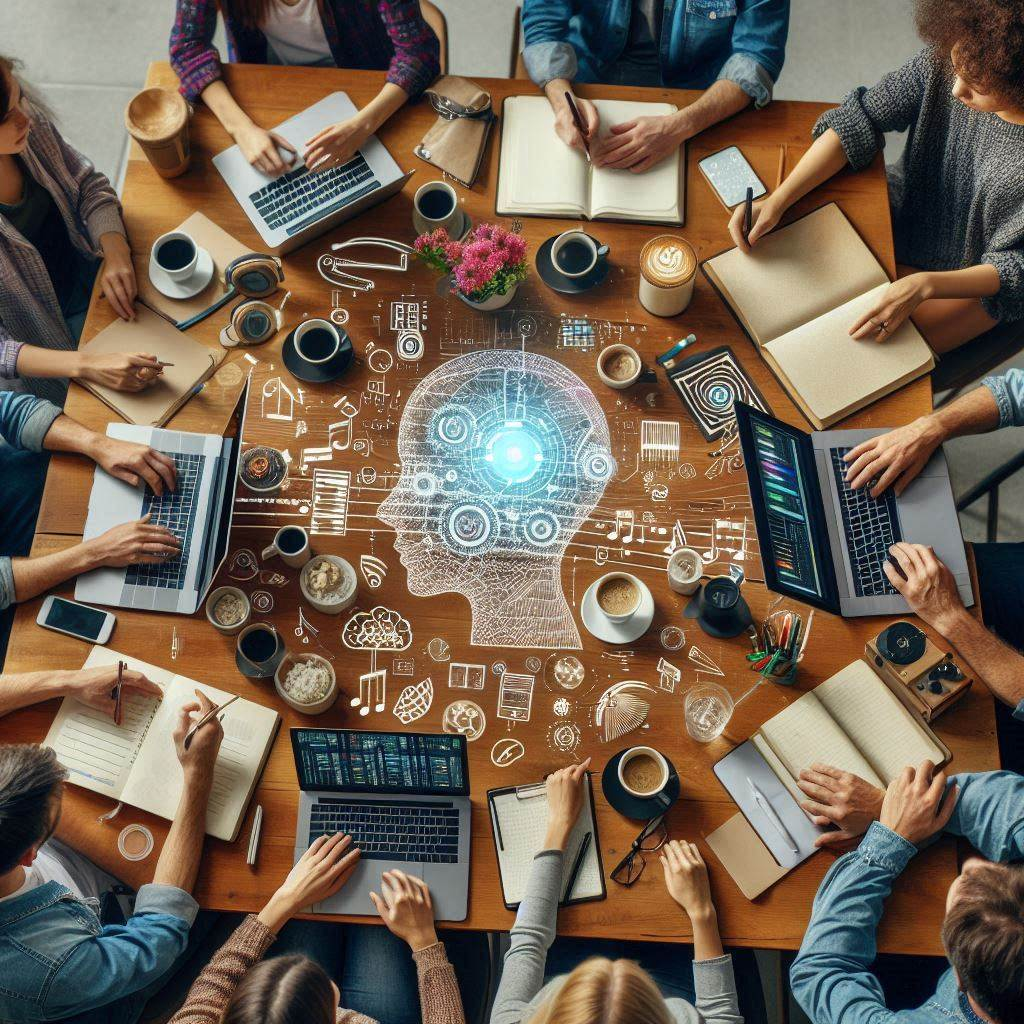
\includegraphics[width=.8\columnwidth]{responsible-ai}%
        %\end{figure}
    %\end{columns}
%\end{frame}
%
%\begin{frame}{challenges}{challenges in (music) ai 2/2}
    %\vspace{-5mm}
    %\begin{columns}
    %\column{.65\linewidth}
        %\begin{itemize}
            %\item   \textbf{sustainability}
                %\begin{itemize}
                    %\item energy consumption
                %\end{itemize}
            %\smallskip
            %\item   \textbf{ownership and copyright}
                %\begin{itemize}
                    %\item protecting rights of content creators while democratizing the creative process
                    %\item navigating complex copyright laws
                    %\item accountability \& liability
                %\end{itemize}
            %\smallskip
            %\item   \textbf{regulatory framework}
                %\begin{itemize}
                    %\item fair use terms
                    %\item transparency and interpretability
                    %\item labeling of ai-created content
                    %\item public perception
                %\end{itemize}
        %\end{itemize}
    %\column{.35\linewidth}
        %\vspace{20mm}
        %\begin{figure}%
            %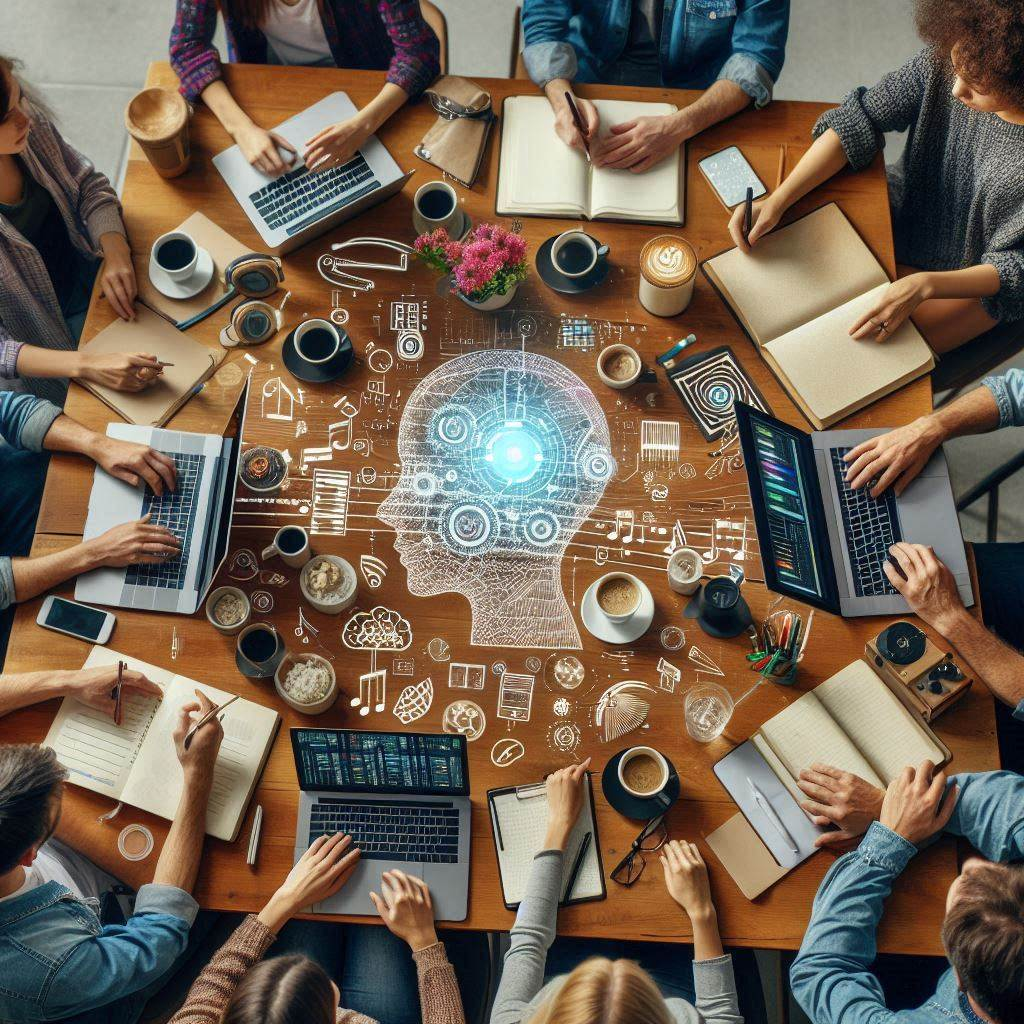
\includegraphics[width=.8\columnwidth]{responsible-ai}%
        %\end{figure}
    %\end{columns}
%\end{frame}
